% Inbuilt themes in beamer
\documentclass{beamer}


%Defining some colours
\definecolor{darkred}{rgb}{0.8,0,0}

% Theme choice: there a number of preset themes to choose from
% Play around with them, Cambridge is nice for first pres
%\usetheme{Szeged}
\usetheme{CambridgeUS} %setting the main theme
\usecolortheme{whale} % setting colour theme
\usefonttheme{professionalfonts} %font theme
\useinnertheme[shadow=true]{rounded}
%\useoutertheme{} %outer theme

%\setbeamertemplate{footline} %Remove footer line in all slides
\setbeamertemplate{navigation symbols}{} %removes navigation symbols
\setbeamertemplate{footline}[page number] %removes footer line, keeps pg#
\setbeamertemplate{caption}{\insertcaption} 


%Setting colours for boxes and captions
\setbeamercolor{block title}{bg=blue!30, fg=black}
\setbeamercolor{block body}{bg=blue!10}
\setbeamercolor{frametitle}{fg=black}

%%%FOR VIDEOS
\usepackage{media9}
\usepackage{multimedia}
\usepackage{graphicx}
% For the Flowchart
%\usepackage{tikz}
%\usetikzlibrary{shapes.geometric, arrows}
%\tikzstyle{startstop} = [rectangle, rounded corners, minimum width=3cm, minimum height=1cm,text centered, draw=black, fill=blue!30]
%\tikzstyle{process} = [rectangle, minimum width=3cm, minimum height=1cm, text centered, draw=black, fill=orange!30]
%\tikzstyle{decision} = [diamond, minimum width=3cm, minimum height=1cm, text centered, draw=black, fill=green!30]
%\tikzstyle{arrow} = [thick,->,>=stealth]

%%% For the Timeline
\usepackage{xcolor}
\usepackage{tikz} \usetikzlibrary{calc, arrows.meta, intersections, patterns, positioning, shapes.misc, fadings, through,decorations.pathreplacing}

\definecolor{ColorOne}{rgb}{0.0,0.5,1.0} %Lightblue
\definecolor{ColorTwo}{rgb}{1.0,0.6,0.4} %lightorange
\definecolor{ColorThree}{rgb}{0.75,0.58,0.89} %lightpurple

% Title page details: 
\title[BEAP Dec 2022]{Double Trouble: Understanding Sex Differences in Synthetic Lethal interactions in Human Cancers \\~\\ Summer Wrap Up} 
\author{Alexander Turco}
\date{August 8, 2023}
\logo{
\includegraphics[height=0.5cm, width=3cm]{logo.png}}

% Bibliography stuff
\usepackage[natbib=true, sorting=nyt, style=authoryear-comp]{biblatex}
\addbibresource{ABC1.bib}

%Extra packages
\usepackage{makecell}


%For itemize
\setbeamertemplate{itemize item}[triangle]

%For Flow Chart
\usepackage{tikz}
\usetikzlibrary{shapes.geometric, arrows}

\tikzstyle{startstop} = [rectangle, 
minimum width=6cm, 
minimum height=1cm,
text centered, 
draw=black, 
fill=blue!30]

\tikzstyle{io} = [trapezium, 
trapezium stretches=true, % A later addition
trapezium left angle=70, 
trapezium right angle=110, 
minimum width=3cm, 
minimum height=1cm, text centered, 
draw=black, fill=blue!30]

\tikzstyle{process} = [rectangle, 
minimum width=3cm, 
minimum height=1cm, 
text align, 
text width=1cm, 
draw=black, 
fill=orange!30]

\tikzstyle{decision} = [diamond, 
minimum width=3cm, 
minimum height=1cm, 
text centered, 
draw=black, 
fill=green!30]
\tikzstyle{arrow} = [thick,->,>=stealth]

\begin{document}
	
	% For my introduction slides, there will be the slide with my title and name as well as an outline slide with the brief overview of what I will discuss.
	% Title page frame - SLIDE 1%%%%%%%%%%%%%%%%%%%%%%%%%%%%%%%%%%%%%%%%%%%%%%%%%%%%%%%%%%%%%%%%%%%%%%%%%%%%%%%%%%%%%%%%%%%%%%%%%%%%%%%%%%%%%%%%%%%%%%%%%%%%%%%%%%%%
	\section{Introduction}
	\begin{frame}
		\titlepage 
		\begin{center}
			%\includegraphics[width=7cm, height=4cm]{cellsatwar.png}
		\end{center}
	\end{frame}
	
	% Remove logo from the next slides
	\logo{}
	
	% Outline frame - SLIDE 2
	\begin{frame}{Overview}
		
		\begin{center}
		\begin{minipage}{6cm}
				
		  		\begin{block}{} Overall Objective and Approach \end{block}
		  		\begin{block}{} Synthetic Lethality Analysis Update \end{block}
		  		\begin{block}{} Limitations of the Study \end{block}
		  		\begin{block}{} Next Steps/Future Work \end{block}
		  		\begin{block}{} Takeaways \& Tips for Future Undergrads \end{block}

		\end{minipage}
		\end{center}
	
	\end{frame}
	
	% For my Background slides, I will talk about important things such as WHat LCRs are, their evolution, stuff like that
	% SLIDE 3 - WHAT ARE LCRs%%%%%%%%%%%%%%%%%%%%%%%%%%%%%%%%%%%%%%%%%%%%%%%%%%%%%%%%%%%%%%%%%%%%%%%%%%%%%%%%%%%%%%%%%%%%%%%%%%%%%%%%%%%%%%%%%%%%%%%%%%%%%%%%%%%%%%
	
	\begin{frame}{Overall Objective}
		\begin{itemize}
			%\includegraphics[width=11cm, height=6cm]{types_of_courses_taken.jpg}
			\item Can we build sex-specific synthetic lethality networks for various cancer types? \newline
			
			\item More specifically, we are trying to elucidate the differences in synthetic lethal interactions between males and females using a network based approach.
		\end{itemize}
	\end{frame}

	%%%%% APPRACH SECTION BEGINS HERE, 2 SLIDES
	
	\section{Approach}
	\begin{frame}{Overall Project Workflow}
		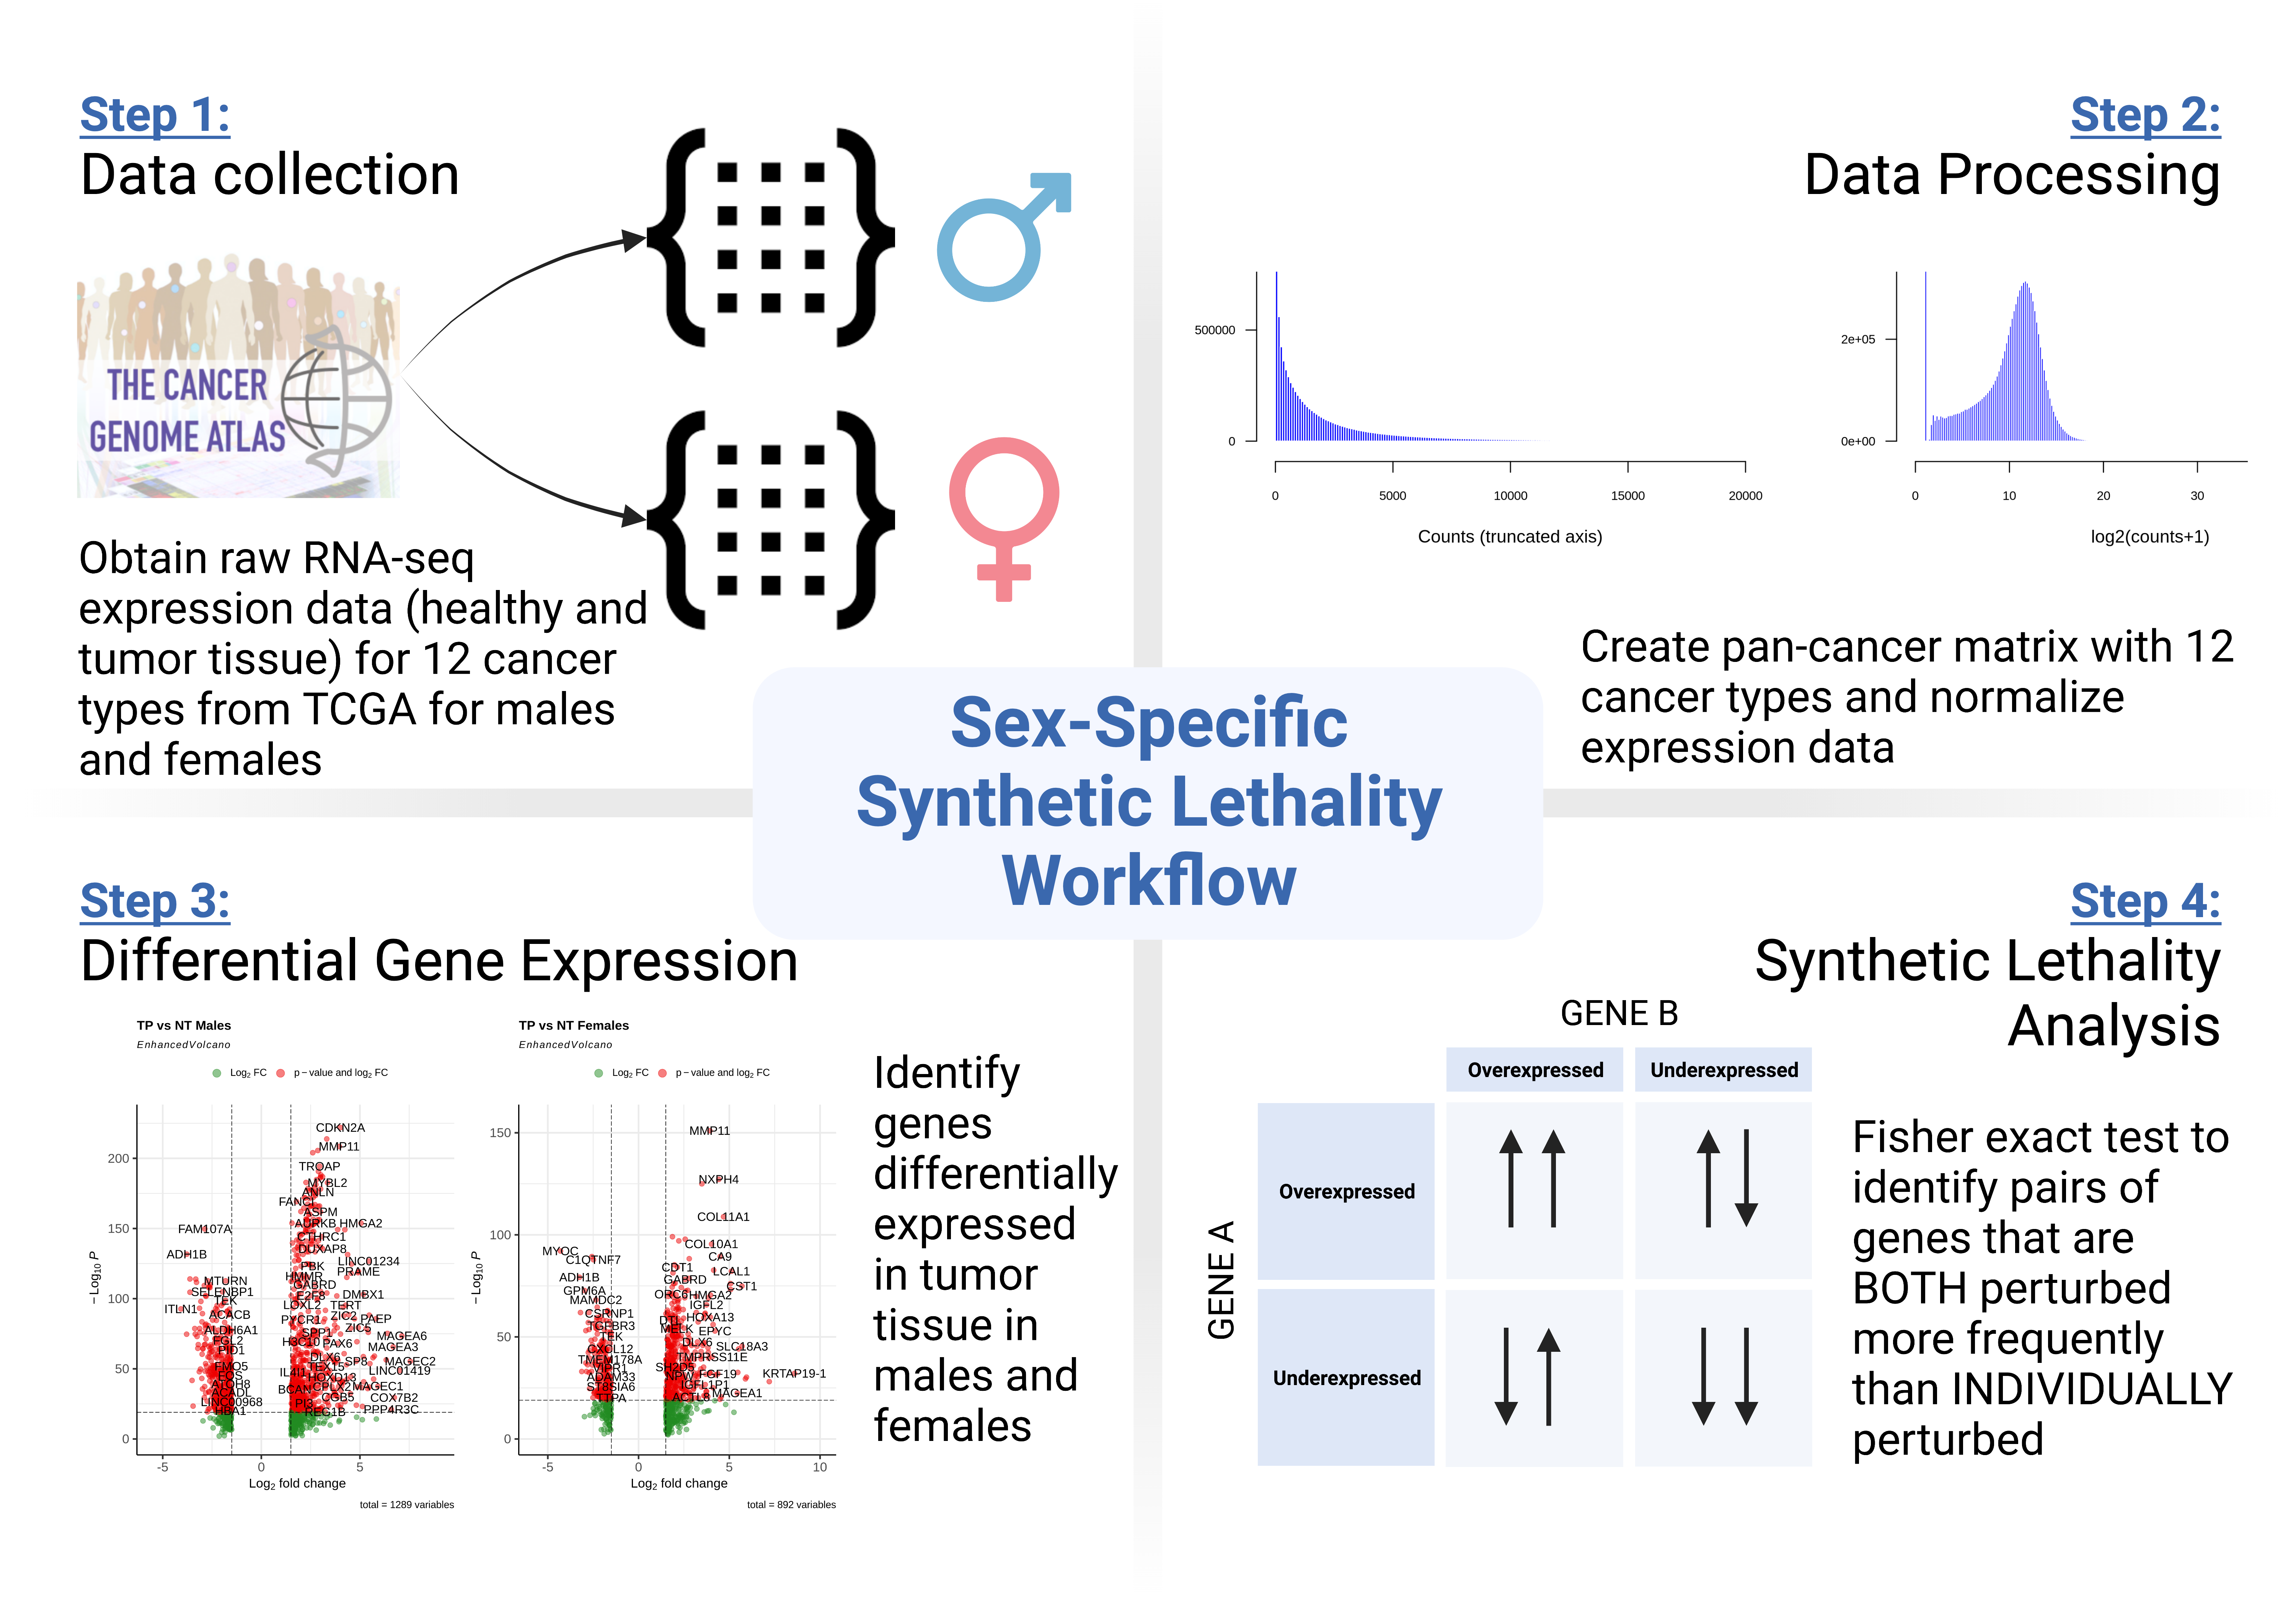
\includegraphics[width=12cm, height=8cm]{project_workflow_slpmcrc_2.png}
	\end{frame}

	\section{Synthetic Lethality}
	\begin{frame}{Using DE Genes to Find Sex-Specific Synthetic Lethal Pairs}
		\begin{center}
			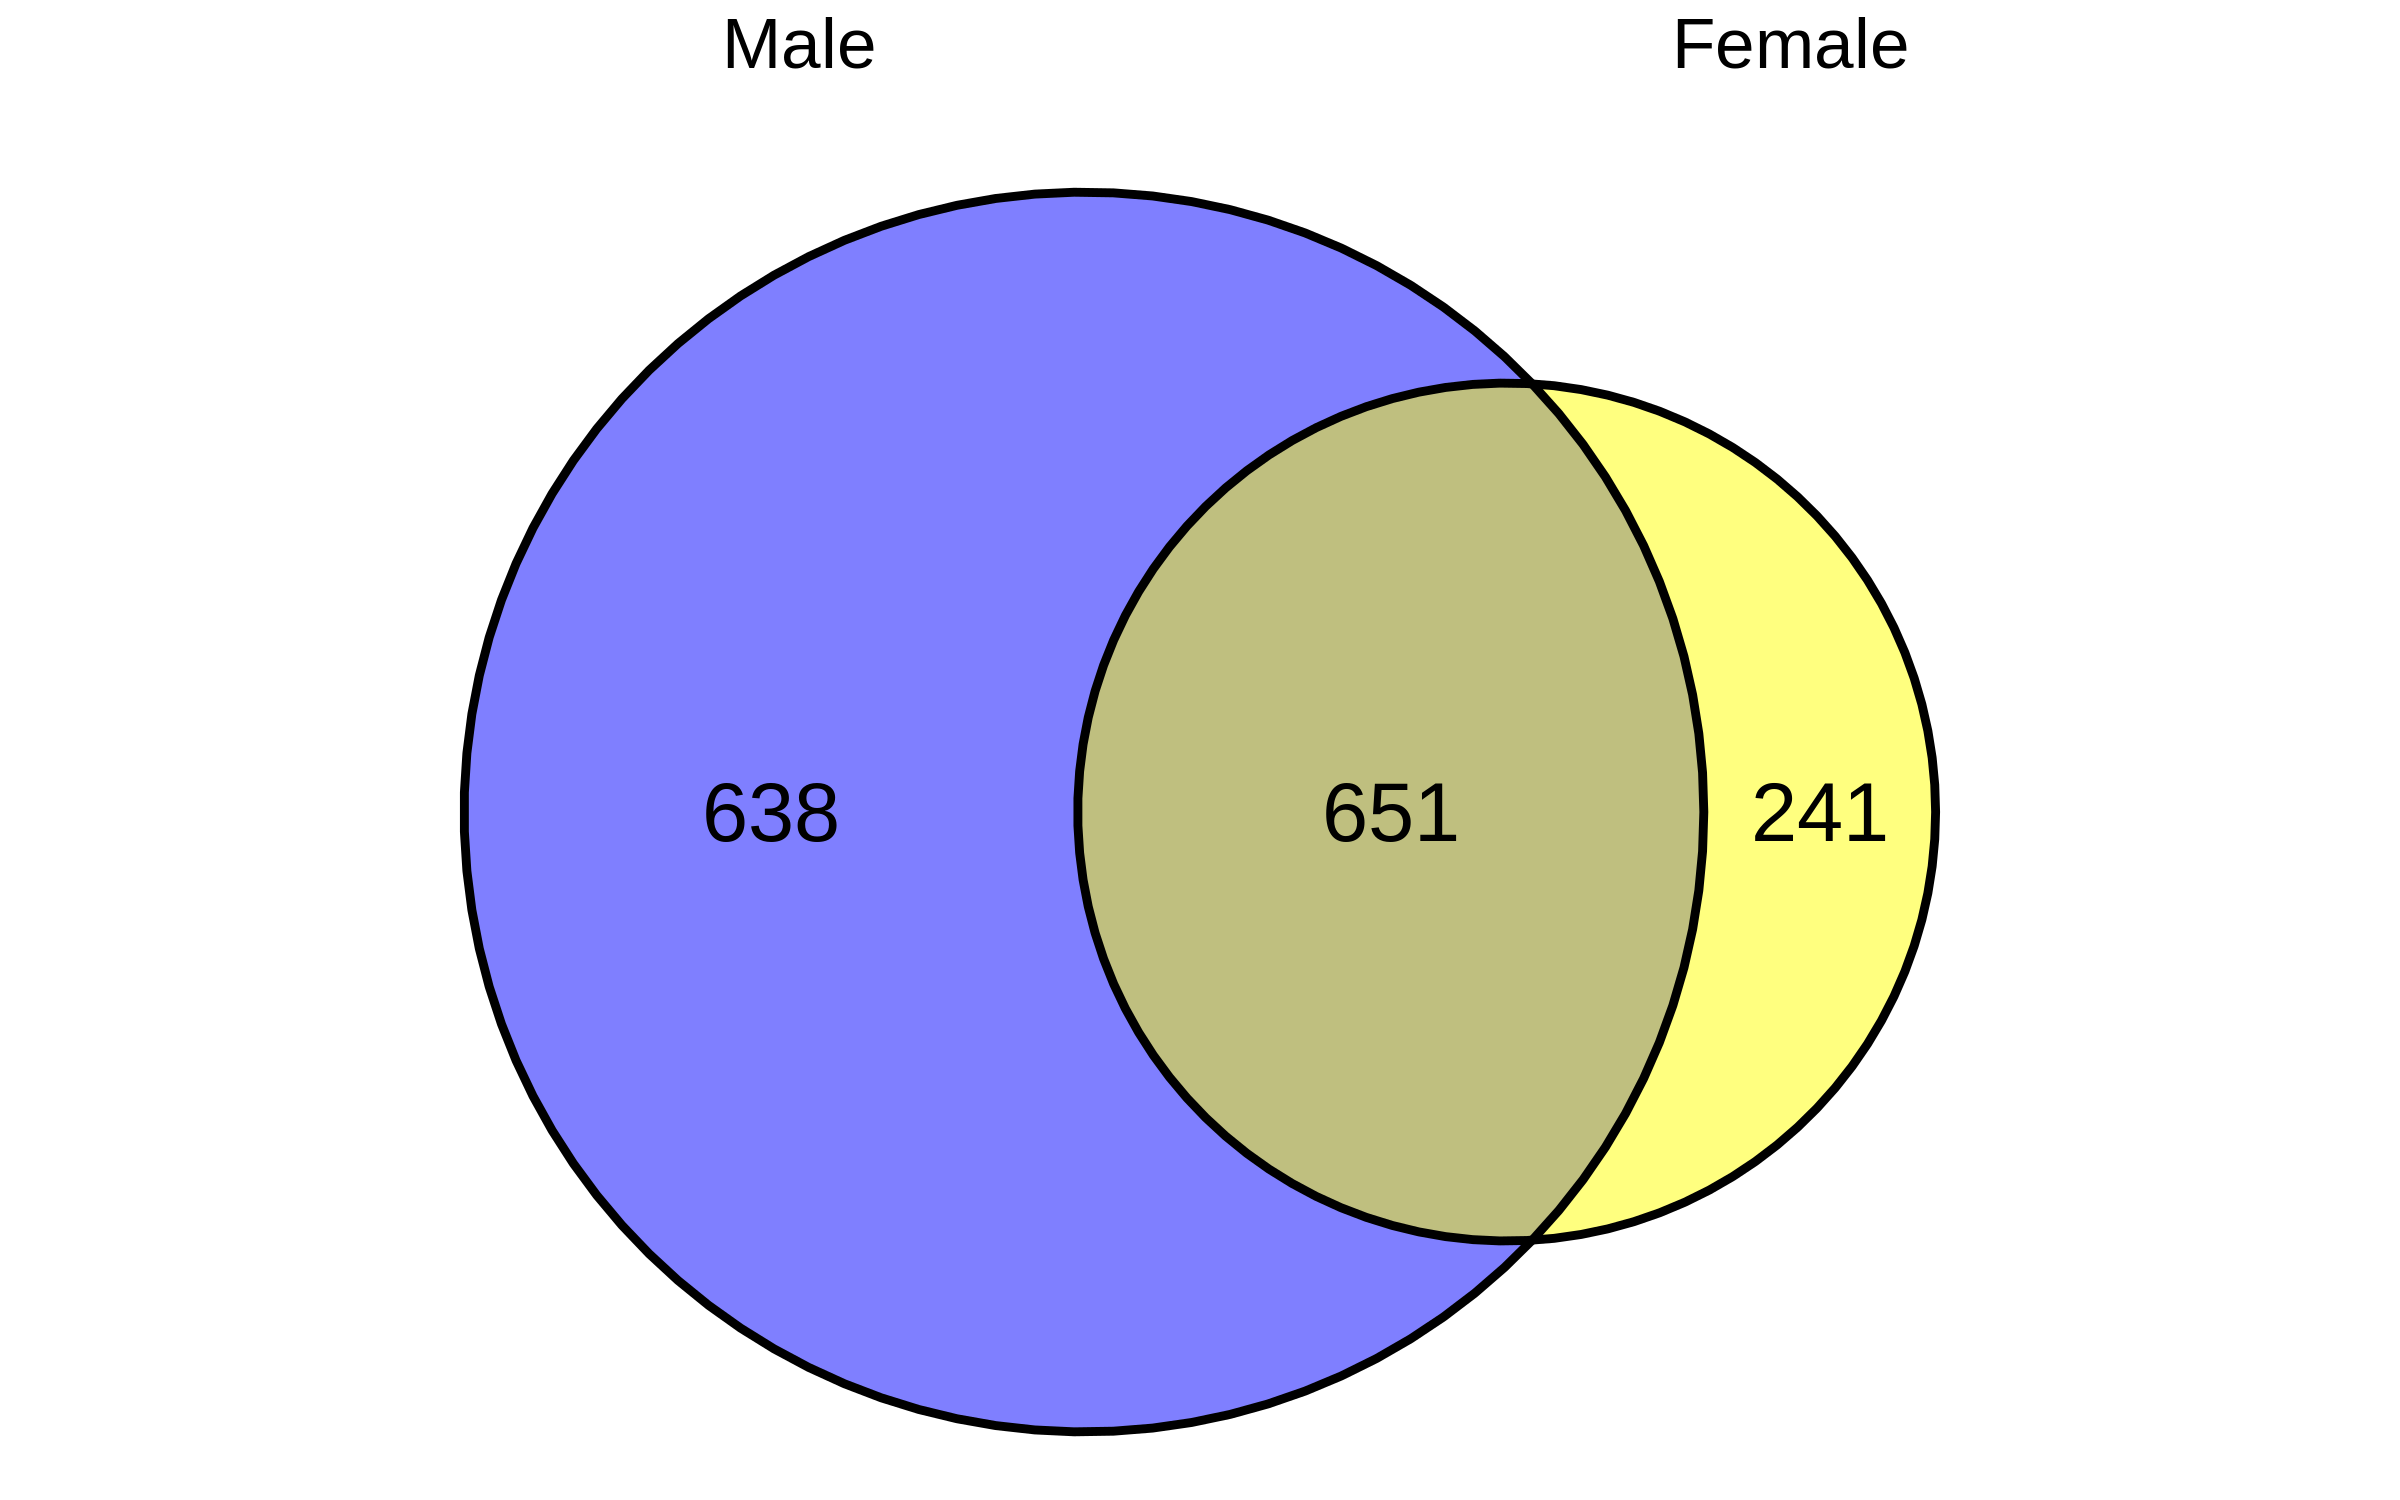
\includegraphics[width=7cm, height=4cm]{all_cancersvenndiagram_malede_vs_femalede_0.9.png}
		\end{center}
		\begin{enumerate}
			\item Find all potential gene pair combinations using differentially expressed genes \newline	
			\textcolor{blue}{${1289 \choose 2 } = 830,116$ Downregulated Male Pairs \newline}
			\textcolor{yellow}{${892 \choose 2 } = 397,386$ Downregulated Female Pairs}
			
			\item Identify pairs of genes that are BOTH perturbed (under and overexpressed) more frequently than INDIVIDUALLY perturbed using Fishers Exact Test
		\end{enumerate}
	\end{frame}

	\begin{frame}{Fishers Exact Test}
		
	\end{frame}
	

\end{document}
